% File: A.tex
% Created: 2014-11-07
% Author: Tesser Paolo
% Email: p.tesser921@gmail.com
% 
%
% Modification History
% Version	Modifier Date	Author			Change
% ====================================================================
% 0.0.1		2014-11-07		Tesser Paolo	inserita sezione
% ====================================================================
% 0.0.2		2015-02-03		Tesser Paolo	sistemata nota Amministratore, Ambiente di lavoro
% ====================================================================
% 0.0.3		2015-03-12		Tesser Paolo	inserito vocabolo: Anamnesi
% ====================================================================
%
\section{A}

\begin{itemize}
	\item \textbf{Ambiente di lavoro}: è ciò che serve ai processi di produzione. \'E composto da:
		\begin{itemize}
			\item persone
			\item ruoli
			\item procedure
			\item infrastrutture
		\end{itemize}
	\noindent
	Esso influisce sulla qualità del processo e del prodotto. Deve essere quindi: completo, ordinato e aggiornato;

	\item \textbf{Amministratore}: è uno dei ruoli di gestione di un progetto. Esso ha il compito di controllare l'ambiente di lavoro e di amministrare le infrastrutture necessarie allo svolgimento del progetto. \newline
	Deve mettere in pratica ciò che le norme chiedono e attraverso sistemi automatizzati le deve fare eseguire senza renderle troppo ingombranti per gli altri membri. Questo lavoro va fatto in maniera preventiva e pro attiva rispetto l'inizio delle attività e del tutto trasparente agli altri componenti. \newline
	A questa figura fanno quindi capo le configurazioni sui sistemi di versionamento e tutta la documentazione che viene redatta. Non attua scelte personali, ma segue quelle concordate con i responsabili;

	\item \textbf{Analisi vs. Progettazione}: [IS] generalmente l'approccio che abbiamo con l'analisi è di tipo top-down in quanto, se non si ha esperienza, non si riescono ad individuare da subito i componenti del sistema. \'E meglio quindi partire dalle richieste del proponente e ricavarne dei casi d'uso e dei requisiti che andranno a raffinarsi sempre di più. \newline
	Per quanto riguarda la progettazione invece si tende ad avere un approccio bottom-up dato che dopo l'analisi si hanno già in mente le componenti principale del sistema. \newline
	Nonostante quanto detto si possono individuare due tipi approccio:
		\begin{itemize}
			\item \textbf{Funzionale}: in questo caso, l'analisi usa prevalentemente il linguaggio naturale, mentre la specifica della progettazione usa linguaggi formali definendo le funzione e il profilo operazionale. Questo implica una progettazione top-down e una programmazione procedurale;
			\item \textbf{Object-oriented}: in questo caso, l'analisi è orientata agli oggetti, ne deriva un uso prevalente di formalismi grafici (Use Case). Questo implica una progettazione bottom-up, basata sul riuso di componenti già esistenti o la realizzazione di componenti riusabili. La programmazione sarà quindi OO.
		\end{itemize}

	\item \textbf{Analista}: è uno dei ruoli di gestione di un progetto. Esso ha il compito di capire il problema per ottenere i requisiti. Non da la soluzione e spesso non segue fino in fondo la realizzazione del progetto, ma è presente principalmente nella fase iniziale. \newline
	Per cercare i requisiti segue un approccio top-down. Parte infatti ad analizzare quelli espliciti del proponente fino a scinderli in vari sottogruppi gerarchici, trovandone nel frattempo anche di impliciti (il numero maggiore tra le due tipologie);

	\item \textbf{Anamnesi}: nella filosofia platonica è quel processo di reminiscenza che, stimolato dalla percezione degli oggetti sensibili, conduce l'uomo a riscoprire gradualmente nel proprio intelletto (attraverso la conoscenza intellettiva) quelle idee eterne che sono causa e origine del mondo fenomenico. La conoscenza sensibile, distinta dalla conoscenza intellettiva, può dunque offrire a quest'ultima lo spunto per avviare un tale processo;

	\item \textbf{Architettura}: [PR] (definizione) Prima degli anni 80 il termine architettura veniva applicato prevalentemente al sistema fisico. Viene riconosciuto anche nell'ambito software dopo l'evento che riconosceva la disciplina stessa del software engineering. \newline
	Viene definita quindi come una collezione di software e componenti del sistema che dialogano tramite connessioni soggette a vincoli. Questo, quando implementate, andranno a soddisfare le necessità degli stakeholders. Un sistema di architettura software comprende:
		\begin{itemize}
			\item l'insieme di decisioni sull'organizzazione del sistema software;
			\item la selezione degli elementi strutturali e la loro interfaccia con il sistema;
			\item la composizione di queste strutture e il comportamento degli elementi in un sempre più ampio sotto insieme;
			\item lo stile architetturale che guida l'organizzazione. Faccio così perché ottengo questo.
		\end{itemize}
		\noindent
	La decomposizione del sistema in componenti deve essere fatta in maniera top-down. I componenti devono anche essere organizzati in modo da definirne ruoli, responsabilità e interazioni. Buone scelte quindi permettono una buona manutenibilità;

	\item \textbf{Architettura della documentazione}: [DOC] TODO
		\begin{figure}[htbp]
			\centering
			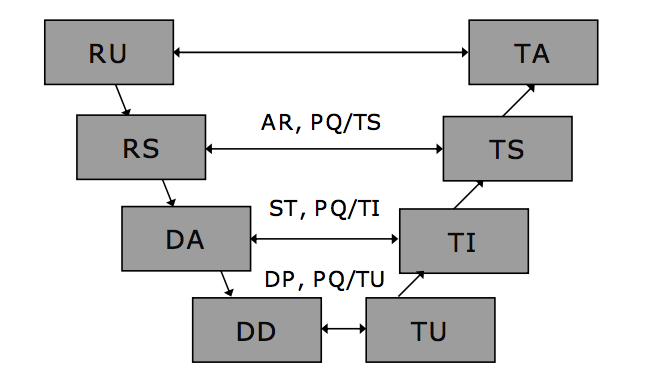
\includegraphics[scale=0.6]{img/v_model_tullio.png}
			\caption{V Model}
			\label{fig:v_model}
		\end{figure}

\end{itemize}
